\chapter{Algorytmy przybliżone}
\label{cha:algorytmy}

Złożoność otaczającego nas świata powoduje, że bardzo często występujące problemy, które chcielibyśmy rozwikłać są w rzeczywistości bardzo trudne do rozwiązania. Dotyczy to praktycznie każdej sfery ludzkiego życia. W wielu sytuacjach natura problemu nie pozwala na zastosowanie metod matematycznych, jednakże nawet w przypadku takich trudności, w których matematyka przychodzi z pomocą, można stwierdzić jedynie, że problem ma rozwiązanie i to nawet najlepsze z możliwych, optymalne, lecz znalezienie go jest praktycznie niewykonalne. Używając języka naukowego, wiele z tych problemów można nazwać NP-trudnymi. Złożoność obliczeniowa algorytmów pozwalających na rozwiązanie ich jest zbyt duża, by w ogóle warto było je stosować. Pojawia się więc potrzeba zastosowania czegoś, co pozwoli na znalezienie rozwiązania dobrego, przybliżającego chociaż rozwiązanie optymalne. I faktycznie jest grupa algorytmów, które pozwalają na uzyskanie takiego efektu. Są to algorytmy przybliżone, inaczej zwane aproksymującymi.

W przeciwieństwie do problemów optymalizacji, których rozwiązanie jest możliwe do znalezienia w czasie wielomianowym, problemy NP-trudne nie dają ,,punktu wyjścia'' do znalezienia rozwiązania optymalnego. Jednakże, niejednokrotnie istnieje ,,punkt wyjścia'', który pozwala na dojście do rozwiązania znajdującego się w pobliżu rozwiązania najlepszego. W tym sensie algorytmy przybliżone podobne są do algorytmów dokładnych: również polegają na uchwyceniu istoty problemu i następnie na znalezieniu algorytmu, która pozwoli na wykorzystanie jej.

Ogromna ilość problemów, dla których nie jesteśmy w stanie znaleźć rozwiązania optymalnego, przyczyniła się do powstania wielu algorytmów aproksymacyjnych.  Przy tworzeniu algorytmów dąży się do tego, by działały one jak najszybciej. W przypadku rozwiązywania przy ich użyciu problemów niejednokrotnie czas ich działania jest dosyć długi. Jednakże, pozwalają one na znalezienie dobrego rozwiązania w sytuacji, gdy użycie algorytmów dokładnych nie pozwoliłoby uzyskać rozwiązania w ogóle.

Ciekawą rzeczą związaną z algorytmami przybliżonymi jest fakt, że wiele z nich powstało na podstawie obserwacji zjawisk występujących w przyrodzie.

Poniżej zostanie przedstawione kilka algorytmów aproksymujących, podstawowe informacje na ich temat, opisany schemat ich działania, a także to, w jaki sposób przy ich pomocy można by próbować rozwiązać problem QAP.
\section{Particle Swarm Optimization}
\label{sec:PSO}
\subsection{Geneza i opis algorytmu} 
Algorytm Particle Swarm Optimization (PSO), czyli algorytm optymalizacji rojem cząstek, po raz pierwszy został przedstawiony w pracy Jamesa Kennedy'ego i Russella Eberharta w 1995 roku, jako metoda optymalizacji nieliniowych funkcji ciągłych. Metoda powstała w oparciu o przeprowadzane symulacje uproszczonych modeli zachowań społecznych. Inspiracją dla autorów były przeprowadzane przez naukowców komputerowe symulacje zachowań stad ptaków czy ławic ryb.

Zachowania stad ptaków zawsze interesowały naukowców. Chcieli oni dociec w jaki sposób ptaki potrafią, latając w licznych stadach, lecieć w sposób synchroniczny, często zmieniając kierunek lotu czy też błyskawicznie się przegrupowując. Z czasem powstawały różnego rodzaju modele tychże zachowań, programy pozwalające na symulowanie ich. Również ciekawą rzeczą był fakt, że ptaki potrafią znaleźć sobie pożywienie, ominąć zagrożenie, mimo że nie posiadają początkowo wiedzy na ten temat. Pojawiły się tezy, że potrafią one wykorzystać zdobytą wiedzę przez inne osobniki, czy tez poprzednie pokolenia. Dążenie do znalezienia pokarmu, próby unikania sytuacji niebezpiecznych czy drapieżników są czynnikami decydującymi o poprawie \"sytuacji życiowej\" ptaków. Jest to swego rodzaju optymalizacja dokonywana samoistnie przez naturę. Analiza tych zachowań stała się punktem wyjścia do tworzenia algorytmów pozwalających na rozwiązywanie wielu trudnych problemów.

Algorytm PSO w pewien sposób przypomina wspomniane wcześniej symulacje, lecz zawiera też parę istotnych różnic. W klasycznej wersji, algorytm zawiera rój cząstek poruszających się w wielowymiarowej przestrzeni, który inicjowany jest w sposób losowy. Cząstki te reprezentują rozwiązania problemu i scharakteryzowane są swoją prędkością i położeniem. Ruch cząstek w kolejnych iteracjach ma na celu przeszukiwanie przestrzeni rozwiązań. Każda z cząstek zapamiętuje znalezioną przez siebie dotychczas najlepszą pozycję. W oparciu o te pozycje, w każdej iteracji cząstki mają aktualizowaną swoją prędkość i położenie.

Algorytm PSO posiada wiele zalet. Przede wszystkim jest bardzo prosty i wydajny, oraz pozwala na optymalizację wielu różnych funkcji. Aktualizacja prędkości i położenia cząstek wymaga jedynie podstawowych operacji matematycznych. Algorytm nie wymaga również zapamiętywania dużej ilości danych, dlatego jest wydajny z punktu widzenia szybkości działania i nie wymaga wielu zasobów pamięci. Ważną cechą jest również to, że jest on bardzo odporny na wpadnięcie do minimum lokalnego.

\subsection{Model matematyczny algorytmu}
Model matematyczny algorytmu PSO może być przedstawiony w następujący sposób:
\textit{Mamy dany rój cząstek, który składa się z n cząstek. Każda z nich porusza się w d-wymiarowej przestrzeni. Każda z cząstek opisana jest przez dwa wektory:}

\begin{itemize}
\item\textit{wektor położenia:}
\newline
\begin{equation}
x_i = [x_{i1},x_{i2},...,x_{id}]
\end{equation}
\newline
\item\textit{wektor prędkości:}
\newline
\begin{equation}
v_i = [v_{i1},v_{i2},...,v_{id}]
\end{equation}
\newline
\end{itemize}

\textit{Ponadto, każda z cząstek zapamiętuje znalezioną przez siebie najlepszą dotychczas pozycję w wektorze:}
\newline
\begin{equation}
x_i^b=[x_{i1}^b,x_{i2}^b,...,x_{id}^b]
\end{equation} 
\newline
\textit{Zapamiętywana jest również w wektorze $x^*$ najlepsza dotychczas pozycja w ogóle znaleziona przez wszystkie cząstki w roju.}

\textit{Wartości prędkości i położenia w każdej iteracji algorytmu aktualizowane są odpowiednio według poniższych wzorów[odniesienie]:}
\newline
\begin{equation}
v_{ij}(t)=w \cdot v_{ij}(t-1)+c_1\cdot r_1 \cdot (x_{ij}^b(t-1)-x_{ij}(t-1))+c_2 \cdot r_2 \cdot (x_j^*(t-1)-x_{ij}(t-1))
\end{equation}
\newline
\begin{equation}
x_{ij}(t)=x_{ij}(t-1)+v_{ij}(t)
\end{equation}
\newline
\textit{gdzie liczby $r_1$ i $r_2$ są wybierane losowo z przedziału $[0,1]$, natomiast współczynniki $c_1$ i $c_2$ odpowiadają za to, w jakim stopniu do aktualizacji prędkości brane są pod uwagę najlepsze znalezione dotychczas położenia każdej z cząstek z osobna i najlepsze położenie w ogóle. Parametr $w$ określa bezwładność cząstek i z czasem maleje liniowo do $0$.}

\subsection{Pseudokod dla algorytmu PSO}
Poniżej znajduje się pseudokod, który opisuje jak krok po kroku działa algorytm optymalizacji rojem cząstek:
\newpage
\begin{algorithm}[h]
	Wczytaj rozmiar roju n, wymiar d, ilość iteracji t i inne parametry\;
 	\While{nie wystąpił warunek stopu}
 	{
 		$t\leftarrow t+1$\;
  		\For{$i\leftarrow 1$ \KwTo $n$}
  		{
  			Policz dopasowanie cząstki $x_i$\;
  			\If{$x_i$ jest lepsza niż $x_i^b$}
  			{
  				$x_i^b \leftarrow x_i$
  			}
  			\If{$x_i^b$ jest lepsza niż $x^*$}
  			{
  				$x^* \leftarrow x_i^b$
  			}
  		}
  		\For{$i\leftarrow 1$ \KwTo $n$}
  		{
  			\For{$j\leftarrow 1$ \KwTo $d$}
  			{
  				Zaktualizuj prędkość $v_{ij}$\;
  				Zaktualizuj położenie $x_{ij}$\;
  			}
  		}
 	}
 	\caption{Algorytm PSO}
\end{algorithm}

\subsection{Zastosowanie algorytmu PSO dla problemu QAP}
Aby było możliwe zastosowanie algorytmu PSO do rozwiązania problemu przydziału kwadratowego, należy odpowiednio ująć problem QAP, by dało się go wpasować w model algorytmu. Przede wszystkim rozwiązaniami zagadnienia przydziału kwadratowego są permutacje, czyli jest to problem dyskretny. Pozycje cząstek w algorytmie PSO mogą zmieniać się w sposób ciągły, położenie nie musi być określone współrzędnymi całkowitymi. Również w permutacji liczby nie mogą się powtarzać. Natomiast nie stoi nic na przeszkodzie, by zwrócona przez algorytm pozycja cząstki była opisana w każdym kierunku przez współrzędne o tej samej wartości. Proste mapowanie: wartość położenia w $i-tym$ kierunku określa przydzielenie do $i-tej$ lokalizacji obiektu o tejże wartości może powodować, że dany obiekt będzie przydzielony wielokrotnie.
Jedno z możliwych zastosowań algorytmu PSO dla problemu QAP zostało zaproponowane w publikacji [REF]. Dla danych zbiorów obiektów i lokalizacji, odpowiednio:
\newline
\begin{equation}
F=\{F_1,F_2,...,F_n\}
\end{equation}
\newline
\begin{equation}
L=\{L_1,L_2,...,L_n\}
\end{equation}
\newline
tworzy się macierz:
\newline
\begin{equation}
\label{PSO_A}
A=
\begin{bmatrix}
a_{11} & a_{12} & \cdots & a_{1n} \\
a_{21} & a_{22} & \cdots & a_{2n} \\
\vdots & \vdots & \ddots & \vdots \\
a_{n1} & a_{n2} & \cdots & a_{nn} \\
\end{bmatrix}
\end{equation}
\newline
gdzie $a_{ij}$ oznacza stopień przynależności \textit{j-tego} obiektu do \textit{i-tej} lokalizacji. Z racji, iż rozwiązanie jest permutacją, więc do jednej lokalizacji należy przypisać tylko jeden obiekt, muszą być spełnione ograniczenia:
\newline
\begin{equation}
\label{pso_suma_po_i}
\sum\limits_{i=1}^n a_{ij}=1
\end{equation}
\newline
\begin{equation}
\label{pso_suma_po_j}
\sum\limits_{j=1}^n a_{ij}=1
\end{equation}
\newline
oraz
\newline
\begin{equation}
a_{ij} \in \{0,1\}, \; i=1,2,...,n, \; j=1,2,...,n
\end{equation}
\newline

Zastosowanie algorytmu optymalizacji rojem cząstek wymaga zatem przedefiniowania pozycji i prędkości w następujący, bazujący na macierzy \ref{PSO_A}, sposób:
\newline
\begin{equation}
X=
\begin{bmatrix}
x_{11} & x_{12} & \cdots & x_{1n} \\
x_{21} & x_{22} & \cdots & x_{2n} \\
\vdots & \vdots & \ddots & \vdots \\
x_{n1} & x_{n2} & \cdots & x_{nn} \\
\end{bmatrix}
\end{equation} 
\newline
\begin{equation}
V=
\begin{bmatrix}
v_{11} & v_{12} & \cdots & v_{1n} \\
v_{21} & v_{22} & \cdots & v_{2n} \\
\vdots & \vdots & \ddots & \vdots \\
v_{n1} & v_{n2} & \cdots & v_{nn} \\
\end{bmatrix}
\end{equation}
\newline
przy czym, by spełnione były ograniczenia \ref{pso_suma_po_i} i \ref{pso_suma_po_j} stosuje się normalizację macierzy położenia:
\newline
\begin{equation}
X_norm=
\begin{bmatrix}
\frac{x_{11}}{\sum\limits_{i=1}^n x_{i1}} & \frac{x_{12}}{\sum\limits_{i=1}^n x_{i2}} & \cdots &\frac{x_{1n}}{\sum\limits_{i=1}^n x_{in}} \\
\frac{x_{21}}{\sum\limits_{i=1}^n x_{i1}} & \frac{x_{22}}{\sum\limits_{i=1}^n x_{i2}} & \cdots & \frac{x_{2n}}{\sum\limits_{i=1}^n x_{in}} \\
\vdots & \vdots & \ddots & \vdots \\
\frac{x_{n1}}{\sum\limits_{i=1}^n x_{i1}} & \frac{x_{n2}}{\sum\limits_{i=1}^n x_{i2}} & \cdots & \frac{x_{nn}}{\sum\limits_{i=1}^n x_{in}} \\
\end{bmatrix}
\end{equation}
\newline

By uzyskać z macierzy położenia \textit{X} rozwiązanie problemu QAP, w każdej kolumnie macierzy wybierany jest element o największej wartości i przypisywana jest jemu wartość \textit{1}, a pozostałym \textit{0}. PO sprawdzeniu wszystkich kolumn i wierszy otrzymuje się w ten sposób macierz określającą w jaki sposób przypisać obiekty do lokalizacji. Macierz ta spełnia również ograniczenia \ref{pso_suma_po_i} oraz \ref{pso_suma_po_j}.

\section{Algorytm Tabu Search}
\label{sec:TS}
\subsection{Geneza i opis algorytmu}
Algorytm Tabu Search został zaproponowany przez Freda Glovera w roku 1986. Jest to metaheurystyka pozwalająca innym metodom optymalizacji unikać sytuacji, w których te wpadają w minima lokalne. Dzięki metodzie tabu search udało się znaleźć optymalne lub prawie optymalne rozwiązania dla bardzo wielu problemów optymalizacji takich jak szeregowanie zadań, problem przydziału kwadratowego, rozpoznawanie charakteru, kolorowanie grafów.

Słowo tabu kojarzone jest przede wszystkim z czymś zakazanym, najczęściej na tle kulturowym. W przypadku algorytmu należy je rozumieć bardziej jako ograniczenie. W ogólności algorytm tabu search polega na zabranianiu wykonywania danej operacji modyfikującej rozwiązanie zwanej ruchem. Ruch jest funkcją, która transformuje dane rozwiązanie w inne, w przypadku permutacji może to być zamiana miejscami dwóch liczb. W danym momencie możliwy jest pewien podzbiór rozwiązań, w które inne może być przetransformowane. Z dostępnych ruchów wybierany jest ten, który powoduje polepszenie rozwiązania i ostatnio wykonany ruch dodawany jest do tablicy ruchów zabronionych na pewną określoną liczbę iteracji algorytmu. Mechanizm ten pozwalaj na wyjście z minimum lokalnego i pozwala uniknąć ruchów cyklicznych. Jednakże w pewnych określanych sytuacjach możliwe jest wykonanie ruchu zabronionego. Zdefiniowana jest specjalna funkcja, zwana funkcją aspiracji, która pozwala obliczyć, czy zabroniony ruch będzie jednak opłacalny.

Algorytm zatrzymuje się, gdy spełniony jest jeden z warunków zatrzymania. Takimi warunkami mogą być wykonanie z góry założonej iteracji algorytmu czy też wykonaniu ustalonej liczby ruchów, które nie prowadzą do dalszej poprawy rozwiązania.

\subsection{Pseudokod algorytmu Tabu Search}
\begin{algorithm}[H]
	Inicjalizuj pierwsze rozwiązanie x\;
	Inicjalizuj rozwiązanie najlepsze $x^b$: $x^b \leftarrow x$\;
 	\While{nie wystąpił warunek stopu}
 	{
 		Przygotuj listę możliwych ruchów dla obecnego rozwiązania\;
 		Wybierz najlepszy możliwy ruch z uwzględnieniem tablicy tabu i kryterium aspiracji\;
 		Przypisz otrzymane w ruchu rozwiązanie do rozwiązania aktualnego x\;
 		\If{rozwiązanie x jest lepsze od $x^b$}
 		{
 			$x^b \leftarrow x$
 		} 		
 		Zaktualizuj tablicę tabu i kryterium aspiracji\;		
 	}
 	\caption{Algorytm Tabu Search}
\end{algorithm}

\subsection{Zastosowanie algorytmu Tabu Search dla problemu QAP}
Rozwiązaniami problemu przydziału kwadratowego są permutacje określające przydział placówek do lokalizacji. Należy więc, mając dane aktualne rozwiązanie problemu QAP, określić w jaki sposób będzie wykonywany ruch w kolejnych iteracjach działania algorytmu. Zmiana aktualnego rozwiązania musi odbyć się w sposób, który nie spowoduje, że do danej lokalizacji zostanie przypisany więcej niż jeden obiekt, jak również któryś z obiektów nie zostanie desygnowany do żadnego z miejsc. W przeciwieństwie do, przykładowo, algorytmu PSO, strategia Tabu Search pozwala na przeszukiwanie przestrzeni rozwiązań w sposób dosyć prosty. Istnieje wiele metod dokonywania ruchów w przypadku, gdy rozwiązanie jest permutacją. Najczęściej spotykanym w literaturze jest sposób polegający na zamianie miejscem dwóch elementów permutacji. Wynika stąd, że dla permutacji o długości $n$ istnieje $n\choose 2$ kombinacji takiego wyboru. Wykonane ruchu zapisywane są w tablicy tabu i trzymane są w niej przez określoną liczbę iteracji algorytmu. Poniżej znajduje się przykładowa tablica:
\newpage
\begin{figure}[h]
\begin{center}
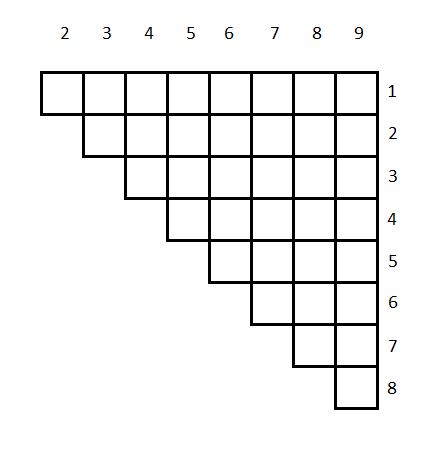
\includegraphics[scale=0.8]{tabu}
\end{center}
\caption{Tablica tabu}
\end{figure}
W powyższej tablicy w komórce o indeksie $(i,j)$ wpisuje się liczbę iteracji algorytmu, podczas których zamiana obiektów o wartości (nie indeksie) nie można zamienić miejscami. Po każdej iteracji liczba ta jest zmniejsza o $1$. Wpis dodawany jest, gdy nastąpiła zamiana miejscami obiektów o wartościach $i$ i $j$.

Innymi metodami pozwalającymi na wykonanie ruchu w algorytmie TS są przykładowo wstawienie jednego z elementów permutacji w inne miejsce i przesunięcie pozostałych elementów, czy też inwersja wybranej grupy elementów permutacji o określonej szerokości.

\section{Algorytm mrówkowy}
\label{sec:mrowka}
\subsection{Geneza i opis algorytmu}
Algorytm mrówkowy (Ant Algorithm) został stworzony przez Marco Dorigo, jako metoda rozwiązywania trudnych problemów optymalizacji jakimi są przykładowo problem komiwojażera (TSP - Travelling Salesman Problem), czy problem przydziału kwadratowego QAP. Inspiracją do powstania algorytmu była obserwacja faktycznych, istniejących w naturze, rojów mrówek. Uwagę naukowców przykuło to, że mrówki, które same są dosyć prostymi stworzeniami, działając w grupie potrafią osiągnąć wysoki poziom organizacji, żyją w zhierarchiwizowanym społeczeństwie. Również ciekawą cechą w zachowaniu mrówek jest to, że nastawione są bardziej na przeżycie całej społeczności niż pojedynczego osobnika. Posiadają one także niespotykane umiejętności pozwalające im na znajdywanie najkrótszej drogi pomiędzy mrowiskiem a miejscem, w którym znajduje się pożywienie.

Ważnym czynnikiem, pozwalającym na znajdywanie najkrótszej ścieżki do źródła pokarmu oraz zapamiętywania tejże drogi, są substancje chemiczne wydzielana przez mrówki, zwane feromonami. Insekty te mają zdolność wyczuwania feromonów i dzięki temu najprawdopodobniej potrafią wybrać drogę, dla której stężenie feromonów jest największe. Pozwala to również innym osobnikom, na wykorzystanie informacji o lokacji pożywienia zdobytej przez inne mrówki. Im częściej dana ścieżka jest uczęszczana przez mrówki, tym większe stężenie feromonów. Mrówki będą zatem korzystać z dróg, na których feromony są bardziej wyczuwalne. Również idąc drogą o mniejszym stężeniu feromonów, mrówki po wyczuciu ich większego stężenia na innej trasie, skierują się na nią tworząc, poprzez zostawianie tegoż związku chemicznego, nowe połączenia. Można w związku z powyższym metaforycznie stwierdzić, że mrówki posiadają zdolność wychodzenia z minimów lokalnych i wybierają minimum globalne.

Z pierwotnych założeń o algorytmach mrówkowych, wyewoluowała cała rodzina algorytmów mrówkowych, rozszerzając w ten sposób ilość problemów, które można dzięki nim rozwiązać. 

\subsection{System mrówkowy - Ant System (AS)}
Jednym z możliwych algorytmów mrówkowych jest system mrówkowy. Jest to pierwszy algorytm bazujących na optymalizacji kolonii mrówek (ACO). Na jego podstawie zostało później opracowanych wiele innych algorytmów. Podczas wypracowywania rozwiązania problemu QAP mrówka określa z pewnym prawdopodobieństwem, który obiekt przypisać do danej lokalizacji. Prawdopodobieństwo to można wyznaczyć z poniższego wzoru[FILIPOWICZ]:
\newline
\begin{equation}
p_{ij}^k(t)=\frac{[\tau_{ij}(t)]^\alpha\cdot[\eta_{ij}]^\beta}{\sum\limits_{l\in N_i^k} [\tau_{il}(t)]^\alpha\cdot[\eta_{il}]^\beta}, \; j \in N_i^k
\end{equation}
\newline
gdzie $\alpha$ i $\beta$ są parametrami  określającymi odpowiednio wagę śladu feromonowego $\tau_{ij}$ i wartości heurystycznej $\eta_{ij}$, a $N_i^k$ jest tzw. sąsiedztwem \textit{-tego} węzła, czyli zbiorem pozostałych wolnych pozycji, do których nie zostały jeszcze przydzielone żadne obiekty.

Ślad feromonowy jest aktualizowany w następujący sposób:
\newline
\begin{equation}
\tau_{ij}(t+1)= \rho \cdot \tau_{ij}(t)+\sum\limits_{k=1}^m \Delta \tau_{ij}^k
\end{equation}
\newline
gdzie $\rho$ jest współczynnikiem wyparowywania feromonów zostawianych przez mrówki, a $\Delta_{ij}^k$ określone jest wzorem:
\newline
\begin{equation}
\Delta \tau_{ij}^k = \left\{ \begin{array}{ccc} \frac{Q}{J^k}, \; gdy \; obiekt \; i \; jest \; przypisany \; do \; lokalizacji \; j \\ 0, \; w \; przeciwnym \;  przypadku \end{array} \right.
\end{equation}
\newline
gdzie $J^k$ jest funkcją celu, a parametr \textit{Q} określa ile feromonów zostawia mrówka.

Obliczenie informacji heurystycznej wymaga wykorzystania dwóch wektorów: \textit{a}, którego \textit{i-ty} element jest sumą odległości lokalizacji \textit{i} do pozostałych lokalizacji, a także wektora \textit{b}, którego \textit{i-ty} element jest analogiczną sumą przepływów. Na podstawie tych wektorów wyznaczana jest macierz E:
\newline
\begin{equation}
E=b \cdot a^T.
\end{equation}
\newline
Dzięki tej macierzy zwiększane jest prawdopodobieństwo przypisania do lokalizacji znajdujących się blisko siebie obiektów o dużym przepływie.

Obiekty oraz lokalizacja, które zostały już przydzielone, zostają zablokowane dopóki rozwiązanie problemu QAP nie zostanie ukończone.

\subsection{Algorytm MMAS}
Algorytm MMAS - \textit{max - min ant system} jest modyfikacją systemu mrówkowego z wprowadzeniem minimalnego i maksymalnego poziomu feromonów. W tej wersji algorytmu tylko jedna, najlepsza globalnie lub w danej iteracji z mrówek zostawia za sobą ślad feromonów. Inicjując algorytm każdy ze śladów feromonowych jest ustawiany na maksymalną wartość $\tau_{max}$. Następnie, podobnie jak w omówionym wcześniej systemie mrówkowym, mrówki przydzielają do nie wybranych jeszcze lokalizacji nieprzydzielone obiekty z pewnym prawdopodobieństwem, które określone jest dla \textit{k-tej} mrówki w następujący sposób:
\newline
\begin{equation}
p_{ij}^k(t)=\frac{\tau_{ij}(t)}{\sum\limits_{l\in N_i^k} \tau_{il}(t)}, \; j \in N_i^k
\end{equation}
\newline
a uaktualnienie śladu feromonów, który jest przez tę mrówkę zostawiany, uzyskiwane jest z równania:
\newline
\begin{equation}
\tau_{ij}(t+1)=\rho \cdot \tau_{ij}(t)+\Delta \tau_{ij}^{best}
\end{equation}
\newline
gdzie
\newline
\begin{equation}
\Delta \tau_{ij}^{best} = \left\{ \begin{array}{ccc} \frac{1}{J^{best}}, \; gdy \; obiekt \; i \; jest \; przypisany \; do \; lokalizacji \; j \\ 0, \; w \; przeciwnym \;  przypadku \end{array} \right.
\end{equation}
\newline

Oznaczenia w powyższych wzorach są analogiczne, do tych dla systemu mrówkowego.
\section{Algorytmy ewolucyjne}
\label{sec:AE}

Algorytmy ewolucyjne są najogólniej rzecz biorąc algorytmy optymalizacji, które bazują na stopniowym polepszaniu pewnej populacji rozwiązań danego problemu. Z powodzeniem są stosowane od wielu lat do rozwiązywania wielu zarówno praktycznych jak i teoretycznych problemów. Istnieje wiele różnorodnych implementacji algorytmów ewolucyjnych. Należą do nich między innymi[evolutionary PDF]:
\begin{itemize}
\item algorytmy genetyczne stworzone przez Johna Henry'ego Hollanda,
\item strategie ewolucyjne opracowane przez Ingo Rechenberga oraz Hansa Paul Schwefela,
\item programowanie ewolucyjne stworzone przez Lawrence'a Fogela.
\end{itemize}

Algorytmy ewolucyjne posiadają wiele cech, które odróżniają je od innych metod optymalizacji. Przede wszystkim zmianom poddawana jest zakodowana w łańcuchu znaków postać problemu , a nie jego parametry bezpośrednio i wykorzystywane jest doświadczenie poprzednich pokoleń. Łańcuch ten ma ustaloną długość i korzysta ze znaków ze skończonego alfabetu. Jak już zostało to wspomniane wcześniej, przetwarzana jest też pewna populacja rozwiązań, nie jedno. By ocenić dane rozwiązanie potrzebna jest jedynie funkcja celu, bądź też coś, co pozwoli porównać dwa rozwiązania i wyłonić lepsze z nich. Kolejnym elementem, który cechuje algorytmy ewolucyjne jest fakt, że stosowane są w nich niedeterministyczne, probabilistyczne reguły wyboru.

Algorytmy genetyczne są chyba najczęściej stosowanymi i najbardziej znanymi implementacjami algorytmów ewolucyjnych. Często, choć niepoprawnie, terminy \textit{algorytmy ewolucyjne} oraz \textit{algorytmy genetyczne} stosowane są zamiennie. Z powodu ich popularności, dalsza część rozdziału będzie poświęcona tejże podgrupie algorytmów ewolucyjnych.

\subsection{Geneza i opis algorytmów genetycznych}
Algorytmy genetyczne zostały opracowane, jak już zostało to wspomniane, przez Johna Hollanda przy pomocy jego kolegów i studentów związanych z Uniwersytetem Michigan. Celami, które im przyświecały podczas tworzenia algorytmów były chęć opisania oraz wyjaśnienie istoty zjawisk zachodzących w świecie przyrody, dzięki którym możliwa jet adaptacja do różnych warunków, a także utworzenie oprogramowania mogącego symulować mechanizmy obecne w systemach biologicznych. Ważną cechą rzeczywistych systemów biologicznych jest odporność tych systemów. Potrafią one szybko zaadaptować się do zmieniających się warunków ich otaczających, posiadają duże zdolności regeneracyjne. Niewątpliwie są to cechy pożądane także przy projektowaniu różnego rodzaju systemów: inżynierskich, ekonomicznych. Skoro algorytmy genetyczne pojawiły się w oparciu o symulacje zjawisko zachodzących w naturze, może pojawić się pytanie czy one same posiadają podobne zdolności. Odpowiedź na nie podał Holland w roku 1975 udowadniając, że algorytmy genetyczne są odporną metodą poszukiwania rozwiązań nawet w skomplikowanych przestrzeniach. Inną ważną zaletą algorytmów genetycznych jest to, że stosowanie ich nie wymaga spełniania założeń dotyczących przestrzeni poszukiwań jakimi są przykładowo ciągłość czy różniczkowalność. Dzięki stosowaniu probabilistycznych technik wyboru, a także dzięki przetwarzaniu całej populacji rozwiązań, w przeciwieństwie do wielu innych analitycznych metod optymalizacji, zmniejszona znacznie jest szansa na zatrzymanie się w ekstremum lokalnym. W tym sensie metody analityczne przejawiają swój brak odporności.
Jednakże, z faktu, iż algorytm genetyczny jest metodą przybliżoną, w przypadku optymalizowania wielu problemów nie jest możliwe stwierdzenie, czy znalezione rozwiązanie, zwrócone przez algorytm jest optymalne i jak daleko znajduje się od optimum. Nie można również zagwarantować, że start algorytmu przy pewnych początkowych ustawieniach zawsze zwróci ten sam rezultat.

W klasycznej, najprostszej wersji, algorytm genetycznych składa się z kilku podstawowych operacji. Mając wygenerowaną losowo populację początkową uruchamiamy algorytm na określoną liczbę operacji. W każdej iteracji dokonujemy oceny każdego z rozwiązań w populacji i w oparciu o ich wartość dopasowania rozwiązań dokonujemy selekcji osobników, na których będą wykonane operacje krzyżowania oraz mutacji. W zależności od postaci rozwiązania, a także od metody jego kodowania, operatory genetyczne mogą działać w różnoraki sposób. W ogólnym przypadki, krzyżowanie polega na wymianie informacji pomiędzy osobnikami wybranymi na drodze selekcji, a mutacja na losowej zmianie wybranego rozwiązania, mogącej zmienić dane rozwiązanie na lepsze bądź gorsze. Teoretycznie z każdą iteracją, ogólne dopasowanie całego pokolenia powinno się polepszać. Ogólną ideą algorytmu jest przetrwanie najsilniejszych i eliminacja słabszych.

\subsection{Operatory selekcji}
Już sam sposób doboru osobników, które posłużą za podstawę dla kolejnego pokolenia, ma kluczowe znaczenie. Istnieje wiele sposobów wyboru rozwiązań. Do takich metod można zaliczyć między innymi:
\begin{itemize}
\item metoda ruletki,
\item metoda rankingowa,
\item metoda turniejowa,
\item metoda progowa.
\end{itemize}

Metoda ruletki polega na "kręceniu" wirtualną ruletką, na której każde z rozwiązań z aktualnej populacji ma wyznaczony swój wycinek koła. Szerokość wycinka zależy od dopasowania danego rozwiązania. Dla każdego rozwiązania jest liczona wartość funkcji dopasowania, a także liczona jest suma wszystkich wartości dopasowania. Stosunek wartości dopasowania danego osobnika do sumy wszystkich dopasowań wyznacza szerokość wycinka ruletki dla danego rozwiązania. Metoda ta faworyzuje osobniki lepsze, nie pozbawiając jednak szansy wyboru tych gorszych. Jednak może to prowadzić w sytuacji, gdy jedno z rozwiązań jest wyraźnie lepsze od pozostałych, że osobniki wybrane do krzyżowania będą się składać głownie z tego jednego.

Metoda bazująca na rankingu rozwiązań nieco zmniejsza rolę dopasowania danego rozwiązania w kontekście jego szans do bycia wybranym na rodzica. W tej metodzie rozwiązania są szeregowane według swojego dopasowania, a o prawdopodobieństwie wyboru decyduje pozycja w rankingu. W oparciu o ranking definiuje się funkcję, która określa ile kopii danego rozwiązania jest brane pod uwagę. W tym sposobie dysproporcje między prawdopodobieństwami wyboru rozwiązań są mniejsze w stosunku do metody ruletkowej.

Metoda turniejowa polega na losowym wyborze dwóch rozwiązań z populacji i rozwiązanie lepsze z tej pary jest brane pod uwagę w dalszych operacjach. Rozwiązania lepsze mają taką samą szansę bycia wybranym do porównania co te słabsze, lecz i tak w przypadku pojedynku, to one wygrają.

Metoda progowa dozwala na losowy wybór rozwiązań z tych, których wartość dopasowania przekracza określony próg. W tej metodzie zawsze pewna pula rozwiązań będzie od razu wykluczona z możliwości do dalszej reprodukcji. Istnieje więc ryzyko, iż pewne rozwiązania, które mogą posiadać obiecujące fragmenty, lecz ogólnie są gorsze od pozostałych rozwiązań w populacji, zostaną odrzucone, a cenna informacja, którą posiadają na drodze poźniejszego krzyżowania nie będzie mogła być wykorzystana.

Należy również wspomnieć, że funkcja dopasowania powinna zwracać liczby nieujemne i dla rozwiązania lepszego jego wartość dopasowania powinna być większa, niż dla gorszego. Nie zawsze da się taką informacje uzyskać bezpośrednio z funkcji celu. Znana jest własność dualności zadań minimalizacji kosztu i maksymalizacji zysku, lecz w przypadku funkcji przystosowania, zwracana wartość zawsze musi być nieujemna. Z tego powodu należy dokonać przekształcenia funkcji celu w funkcję dopasowania. Najczęściej  dokonywane to jest poprzez odejmowanie wartości funkcji celu od pewnej liczby. Jeśli taka różnica jest ujemna, zwracamy 0. Wartość tej liczby może być ustalona w wieloraki sposób. Przykładowo, może to być z góry ustalona liczba, może też być modyfikowana wraz z kolejnymi iteracjami algorytmu, np. może przyjąć wartość największej znalezionej do tej pory wartości funkcji celu.

\subsection{Operatory krzyżowania}
Celem operatorów krzyżowania, zwanych inaczej mieszania, jest spowodowanie wymiany informacji pomiędzy wybranymi rozwiązaniami i utworzenie na tej podstawie kolejnych. Mając wyselekcjonowaną populacje rozwiązań, łączymy w pary osobniki i dokonujemy ich krzyżowania. To w jaki sposób zostanie to wykonane zależy od postaci rozwiązania. Istnieje wiele różnych metod krzyżowania. Inne są wykorzystywane dla rozwiązań kodowanych w sposób binarny, inne dla kodów wykorzystujących liczby rzeczywiste itp. Do najbardziej znanych metod krzyżowania należą:
\begin{itemize}
\item krzyżowanie jednopunktowe,
\item krzyżowanie wielopunktowe,
\item krzyżowanie z częściowym odwzorowaniem PMX,
\item krzyżowanie cykliczne CX,
\item krzyżowanie z zachowaniem porządku OX.
\end{itemize}

Trzy ostatnie z wymienionych operatorów dotyczy rozwiązań będących permutacjami i ich użycie pozwala na zachowanie tej postaci po dokonaniu krzyżowania. Operatory jednopunktowy i wielopunktowy powodują wymianę pomiędzy osobnikami fragmentów kodu pomiędzy wylosowanymi punktami. Operacja krzyżowania wykonywana jest z pewnym określonym jako parametr algorytmu prawdopodobieństwem. Dla każdego z rozwiązań, wybranych na drodze selekcji, losowane jest czy będzie brane pod uwagę w dalszych działaniach. W zależności od przyjętych założeń, może zaistnieć potrzeba doboru dodatkowych rozwiązań w przypadku, gdy jest ich niewystarczająca ilość, by móc dokonać operacji krzyżowania.

\subsection{Operatory mutacji}
Operacja mutacji jest losową zmianą dokonywaną na rozwiązaniach wzorowaną na mutacjach występujących faktycznie w przyrodzie. Jest ona błądzeniem przypadkowych w przestrzeni ciągów kodowych[goldberg]. Operator mutacji pozwala na przywrócenie utraconych ważnych informacji w kodzie rozwiązania, bądź na uzyskanie dobrych (lub złych) cech w rozwiązaniu, których często nie dałoby się otrzymać na drodze krzyżowania. Z racji iż prawdopodobieństwo wystąpienia mutacji jest wielokrotne mniejsze niż wystąpienie krzyżowania, operacja ta odgrywa drugorzędną rolę w działaniu algorytmu, choć niejednokrotnie pozwala na uzyskanie zaskakujących rezultatów.

W przypadku binarnej postaci kodu rozwiązań operacja mutacji najczęściej polega na zamianie wartości bit z $0$ na $1$ i na odwrót. W innych przypadkach mutacja polega na zmianie wybranego elementu na inny dopuszczalny. W sytuacji, gdy rozwiązaniem jest permutacja, należy zadbać, by operator mutacji pozostawiał rozwiązanie w poprawnej postaci. Mutacja w takim przypadku może polegać przykładowo na zamianie miejscami dwóch elementów, czy też na inwersji pewnego fragmentu kodu. 

\subsection{Schemat działania algorytmu genetycznego}
Poniżej znajduje się pseudokod dla klasycznej wersji algorytmu genetycznego:
\begin{algorithm}[H]
	Inicjalizuj populację początkową\;
 	\While{nie wystąpił warunek stopu}
 	{
 		Dokonaj selekcji rozwiązań będącej podstawą dla nowego pokolenia;\
 		Dokonaj operacji krzyżowania na wybranych osobnikach\;
 		Dokonaj operacji mutacji na osobnikach otrzymanych na drodze krzyżowania\;
 		Zaktualizuj populację w oparciu o otrzymane rozwiązania w wyniku działania operatorów genetycznych
 	}
 	\caption{Algorytm genetyczny}
\end{algorithm}
\subsection{Zastosowanie algorytmu genetycznego dla problemu QAP}
Algorytm genetyczny można w łatwy sposób zaimplementować dla problemu QAP. Postać rozwiązania problemu przydziału kwadratowego to permutacja. Należy więc na każdym etapie działania algorytmu dokonywać zmian w taki sposób, by zwracane w kolejnych iteracjach populacje rozwiązań były populacjami permutacji. Wyżej zostały wymieniowe metody krzyżowania, takie jak operatory OX, PMX, CX, i mutacji, które mogą być stosowane dla rozwiązań permutacyjnych.
Optymalizacja problemu QAP polega na minimalizacji kosztu przydziału obiektów do lokalizacji. Z tego powodu funkcja celu (wzór) nie nadaje się wprost do oceny przystosowania osobników. Funkcję dopasowania można więc uzyskać z funkcji celu poprzez odejmowanie wartości funkcji celu od pewnej liczby, którą może być największa znaleziona dotychczas wartość funkcji celu, czy też najgorsza wartość dopasowania w ostatniej iteracji itp.